%本稿で対象とするプラットフォームでは、複数のGPUタスクが存在し、複数のGPUカーネルが同一タスクに存在することを想定している。
%そのため複数のGPUカーネルと一般的に同期に利用されるCUDA APIの$cuCtxSynchronize()$の回数は一対一で対応付けされずに、
%複数のGPUカーネルの発行を一度の$cuCtxSynchronize()$によって同期する可能性がある。
%そのため、$cuCtxSynchronize()$を用いた同期ベースなスケジューリングを行うにあたり、各GPUカーネルの終了と同期のために、アプリケーション自体の変更を必要とするため好ましくない。

%本問題に対してGPUSyncではNOTIFYに限って対処しており、$LITMUS^{RT}$の拡張という形でLinuxの割込みのbottom-halfであるtaskletをカーネル内部で傍受し、
%コールバック関数の引数のポインタが指すメモリスペースによって、どのGPUからの割込みかを判断している。
\if 0
その手法では、soft-irqを利用しているためレイテンシが大きく、どのカーネルであるかの判断もできない。
GdevではGPUタスクの同期はFENCE、スケジューラの立ち上げはNOTIFYを用いている。
NOTIFYの獲得は、デバイスドライバがカーネルに登録するISRにGdevのコールバック関数を追記することで割込みタイミングを獲得している。
GPUタスクの同期にFENCEを用いている理由としては、あくまでGPUを効率よく扱う点にフォーカスしており、CPU側の処理も含めた効率について考慮していないためである。
ただし,GPUの実行はすべてAPIドリブンであり,CPU側で動作するGPUタスクからGPUカーネルを発行されて実行が行われる.
GPUカーネルの優先度とGPUタスクの優先度が異なるケースはよほど特殊でない限り利用しない(我々の思いつく限り存在しない)ため,
are non-preemptive
カーネル、デバイスドライバの編集無しにスケジューリングするための最も大きな課題は、この同期を獲得し、識別するかといった点である。
\fi

\if 0
本稿で対象とするプラットフォームでは、複数のGPUタスクが存在し、複数のGPUカーネルが同一タスクに存在することを想定している。
そのため複数のGPUカーネルと一般的に同期に利用されるCUDA APIの$cuCtxSynchronize()$の回数は一対一で対応付けされずに、
複数のGPUカーネルの発行を一度の$cuCtxSynchronize()$によって同期する可能性がある。
そのため、$cuCtxSynchronize()$を用いた同期ベースなスケジューリングを行うにあたり、各GPUカーネルの終了と同期のために、アプリケーション自体の変更を必要とするため好ましくない。

本問題に対してGPUSyncではNOTIFYに限って対処しており、$LITMUS^{RT}$の拡張という形でLinuxの割込みのbottom-halfであるtaskletをカーネル内部で傍受し、
コールバック関数の引数のポインタが指すメモリスペースによって、どのGPUからの割込みかを判断している。
その手法では、soft-irqを利用しているためレイテンシが大きく、どのカーネルであるかの判断もできない。
GdevではGPUタスクの同期はFENCE、スケジューラの立ち上げはNOTIFYを用いている。
NOTIFYの獲得は、デバイスドライバがカーネルに登録するISRにGdevのコールバック関数を追記することで割込みタイミングを獲得している。
GPUタスクの同期にFENCEを用いている理由としては、あくまでGPUを効率よく扱う点にフォーカスしており、CPU側の処理も含めた効率について考慮していないためである。
ただし,GPUの実行はすべてAPIドリブンであり,CPU側で動作するGPUタスクからGPUカーネルを発行されて実行が行われる.
GPUカーネルの優先度とGPUタスクの優先度が異なるケースはよほど特殊でない限り利用しない(我々の思いつく限り存在しない)ため,
are non-preemptive
カーネル、デバイスドライバの編集無しにスケジューリングするための最も大きな課題は、この同期を獲得し、識別するかといった点である。
\fi
%GPUの同期は2つの手法がある。
%一つはPollingを用いた方法で本誌ではFENCEと呼ぶ。
%もう一つはInterruptによって同期する方法で本誌ではNOTIFYと呼ぶ。
%これらは両者ともGPUに搭載されたエンジンを用いて行われる。
%GPUには多くのエンジン(マイクロコントローラ)が搭載されている。
%本論文では詳しいアーキテクチャはメインではないので省略するが、詳細は過去の文献\cite{kato:timegraph,fujii:apsys2013}に記載しています。
%このエンジンにはコンテキスト管理用、コマンド受け取り用、データ転送用などが存在している。
%通常、コマンド受け取り用のエンジンが受け取ったコマンドのヘッダから、
%そのコマンドを使用するエンジンへと送信し、処理が行われる。
%この順序はすべてFIFOで行われる。
%FENCEを用いた方式では、まず同期用に仮想アドレス空間にマップされたバッファをGPUメモリに用意する。
%そして、このメモリに値をEngine経由で書き込むためのコマンドを発行する。
%Engineはカーネル実行とメモリ転送終了後に値を書き込むため、
%CPU側でマップされたメモリアドレスをポーリングしながらチェックすれば同期が可能である。
%NOTIFYについてもEngineの機能を利用する。

%タスクはTASK\_INTERRUPTIBLE or TASK\_UNINTERRUPTIBLEにした上でschedule()を呼ぶか、
%waitqueueなどを用いて上記に相当する処理を行いsuspendする。
%そしてEngineから割込みを発生させるコマンドを発行し、割り込みコントローラがそれを獲得、
%GPUドライバが登録した$Interrupt Service Routine$ (ISR) を立ち上げる。
%ISR内では、各割込みに関するステータスをマッピングされたレジスタから読み込み、
%各割込みごとに処理を行う。処理後は割込み完了フラグを書き込み、初期化する。
%Gdevではsynchronization ベースのスケジューリングを行っており、GPUカーネル終了の検知し次のタスクを立ち上げる部分に割込みを用いている。

\if 0
\begin{figure}[t]
\begin{center}
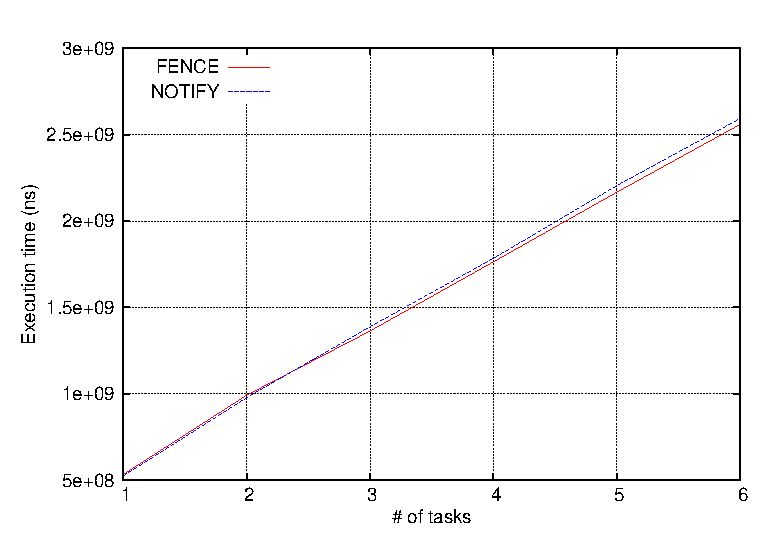
\includegraphics[width=0.35\textwidth]{img/poll_vs_irq}
\caption{FENCE vs NOTIFY}
\end{center}
\label{fig:poll_vs_irq}
\end{figure}
\fi

%二種類の手法が存在する理由としては、FENCEとNOTIFYにそれぞれアドバンテージがあるためである。
%Figure~\ref{fig:poll_vs_irq} shows FENCEを1とした時のNOTIFYのrelative speedである。
%タスクが1つの場合はFENCEがNOTIFYよりも8ms速い結果が出ており、
%タスクが3個に増えた時点でNOTIFYの方が早くなり、タスク6個の時点では33ms速い結果がでている。
%NOTIFYによってタスクがスリープしている間に他のタスクのCPU利用部分が動作することで、
%効率的にGPUタスクが実行できているためである。
%GPUをより効率的に利用するためにはFENCE、NOTIFYをうまく使い分ける必要がある。


\if 0
\textbf{Scheduling policies:}
We discuss the scheduling policies to be equipped as the scheduling foundation.
%ここでは上記スケジューリング基盤として備えるべきスケジューリングポリシーについて議論する。
Generaly, CPU task is sufficient that can priority schedling in the real-time systems.
Priority scheduling are two main categories, that are Fixed Prioriry scheduling (e.g. ratemonotonic, deadline monotonic) and Dinamic Priority scheduling (e.g. Earliest Deadline First:EDF).

%CPU側で動作するタスクに関してはリアルタイムなシステムにおいては、優先度スケジューリング且ができていればよい。
%固定優先度方式としてDeadline-Monotonic (DM)\cite{sched:dm}やRate-Monotonic (RM)\cite{sched:rm}などがあり、
%動的優先度方式としてEarist deadline first (EDF) などがある。

GPU kernele execution is to inconvenience in the prioriry-based scheduling.
GPU kernek is including GPU task, therefore, priority inversion is happend in the case of different the GPU kernel priority and the GPU task kernel priority.
Thus basically, GPU kernel scheduling is appropriate to follow the priority of the process.
Additionally, scheduler need each GPU tasks QoS management.

%GPUカーネルの実行に関しては優先度ベースなスケジューリングでは不都合が生じる。
%GPUカーネルはGPUタスクに含まれるものである。
%そのためGPUカーネルの優先度とGPUタスクの優先度が異なるケースは、その時点でGPUタスクの優先度逆転が発生する。
%したがって、GPUカーネルスケジューリングはプロセスのスケジューリングに沿って実行するのが適正であり、
%それに加えて必要なのが各GPUタスクごとのGPUリクエストに対するQoSを担保することである。

%QoSを担保する方法としてこれまでリソースリザベーションベースのスケジューリングポリシーが提案\cite{gdev,cbs,tbs}されてきており、
The resource reservation-based scheduling policy has been proposed\cite{gdev,cbs,tbs} as a method to guarantee QoS.
This paper adopt the BAND scheduling that gave a certain defree of success in QoS collateral in Gdev.
%本論文ではGdevでGPUのQoS担保に一定の成果を挙げたBANDスケジューリングを利用する。

\fi
\subsection{GPU synchronization}
Section~\ref{sec:system_model}で説明したinterrupt-drivenなスケジューラ起床を実現するために,kernel freeなまま同期に用いるinterruptを取得するinterrupt interceptを実装する.
加えて,runtime environmentに依存しない形でNOTIFY,FENCEを実装することで,
任意の識別子を追記することが可能な同期メカニズムを実現する.

%ラウンチされたカーネルが終了したタイミングをスケジューラはNOTIFYかFENCEによって取得する。
%本ワーカースレッドは実行中のカーネルが終了した時点で次のタスクの選択を行う。
%ワーカースレッドはタスクの選択後にCPU資源を他のタスクに明け渡すためにサスペンドに入る。

\if 0
Linux-RTXG is synchronization based scheduler that need to know the timing of GPU kernel launch request and the timing of it kernel finish.
it timing of GPU kernel launch request is scheduling point that is given by rtx\_gpu\_launch().
In order to notify the completion of the current GPU kernel executin, is able to given synchronization by using NOTIFY/FENCE.
NVIDIA proprietary software can awaken NOTIFY/FENCE by set the flag when create the GPU context.
\fi
%本スケジューラsynchronization basedなスケジューラでありGPUカーネルのラウンチを要求されたタイミングと、そのカーネルが終了したタイミングを知る必要がある。
%Application is 
%Linux-RTXGでは前述のようにrtx\_gpu\_launch()によってGPUカーネルのラウンチ要求を受け取る.
%アプリケーションはrtx\_gpu\_launch()を呼び出すことでioctlシステムコールによって、
%ユーザコンテキストからカーネルコンテキストへと処理が移り、
%スケジューラが保持するGPUタスク情報 (e.g. waiting task status, running task status, GPU device status) を基に自身が動作可能かを確認し動作する。
%スケジューラを通じて、資源を獲得できた場合にはGPUカーネルのラウンチの発行が可能となる。
%be able to issue the GPU kernel launch via Scheduler.
